\documentclass[1p]{elsarticle_modified}
%\bibliographystyle{elsarticle-num}

%\usepackage[colorlinks]{hyperref}
%\usepackage{abbrmath_seonhwa} %\Abb, \Ascr, \Acal ,\Abf, \Afrak
\usepackage{amsfonts}
\usepackage{amssymb}
\usepackage{amsmath}
\usepackage{amsthm}
\usepackage{scalefnt}
\usepackage{amsbsy}
\usepackage{kotex}
\usepackage{caption}
\usepackage{subfig}
\usepackage{color}
\usepackage{graphicx}
\usepackage{xcolor} %% white, black, red, green, blue, cyan, magenta, yellow
\usepackage{float}
\usepackage{setspace}
\usepackage{hyperref}

\usepackage{tikz}
\usetikzlibrary{arrows}

\usepackage{multirow}
\usepackage{array} % fixed length table
\usepackage{hhline}

%%%%%%%%%%%%%%%%%%%%%
\makeatletter
\renewcommand*\env@matrix[1][\arraystretch]{%
	\edef\arraystretch{#1}%
	\hskip -\arraycolsep
	\let\@ifnextchar\new@ifnextchar
	\array{*\c@MaxMatrixCols c}}
\makeatother %https://tex.stackexchange.com/questions/14071/how-can-i-increase-the-line-spacing-in-a-matrix
%%%%%%%%%%%%%%%

\usepackage[normalem]{ulem}

\newcommand{\msout}[1]{\ifmmode\text{\sout{\ensuremath{#1}}}\else\sout{#1}\fi}
%SOURCE: \msout is \stkout macro in https://tex.stackexchange.com/questions/20609/strikeout-in-math-mode

\newcommand{\cancel}[1]{
	\ifmmode
	{\color{red}\msout{#1}}
	\else
	{\color{red}\sout{#1}}
	\fi
}

\newcommand{\add}[1]{
	{\color{blue}\uwave{#1}}
}

\newcommand{\replace}[2]{
	\ifmmode
	{\color{red}\msout{#1}}{\color{blue}\uwave{#2}}
	\else
	{\color{red}\sout{#1}}{\color{blue}\uwave{#2}}
	\fi
}

\newcommand{\Sol}{\mathcal{S}} %segment
\newcommand{\D}{D} %diagram
\newcommand{\A}{\mathcal{A}} %arc


%%%%%%%%%%%%%%%%%%%%%%%%%%%%%5 test

\def\sl{\operatorname{\textup{SL}}(2,\Cbb)}
\def\psl{\operatorname{\textup{PSL}}(2,\Cbb)}
\def\quan{\mkern 1mu \triangleright \mkern 1mu}

\theoremstyle{definition}
\newtheorem{thm}{Theorem}[section]
\newtheorem{prop}[thm]{Proposition}
\newtheorem{lem}[thm]{Lemma}
\newtheorem{ques}[thm]{Question}
\newtheorem{cor}[thm]{Corollary}
\newtheorem{defn}[thm]{Definition}
\newtheorem{exam}[thm]{Example}
\newtheorem{rmk}[thm]{Remark}
\newtheorem{alg}[thm]{Algorithm}

\newcommand{\I}{\sqrt{-1}}
\begin{document}

%\begin{frontmatter}
%
%\title{Boundary parabolic representations of knots up to 8 crossings}
%
%%% Group authors per affiliation:
%\author{Yunhi Cho} 
%\address{Department of Mathematics, University of Seoul, Seoul, Korea}
%\ead{yhcho@uos.ac.kr}
%
%
%\author{Seonhwa Kim} %\fnref{s_kim}}
%\address{Center for Geometry and Physics, Institute for Basic Science, Pohang, 37673, Korea}
%\ead{ryeona17@ibs.re.kr}
%
%\author{Hyuk Kim}
%\address{Department of Mathematical Sciences, Seoul National University, Seoul 08826, Korea}
%\ead{hyukkim@snu.ac.kr}
%
%\author{Seokbeom Yoon}
%\address{Department of Mathematical Sciences, Seoul National University, Seoul, 08826,  Korea}
%\ead{sbyoon15@snu.ac.kr}
%
%\begin{abstract}
%We find all boundary parabolic representation of knots up to 8 crossings.
%
%\end{abstract}
%\begin{keyword}
%    \MSC[2010] 57M25 
%\end{keyword}
%
%\end{frontmatter}

%\linenumbers
%\tableofcontents
%
\newcommand\colored[1]{\textcolor{white}{\rule[-0.35ex]{0.8em}{1.4ex}}\kern-0.8em\color{red} #1}%
%\newcommand\colored[1]{\textcolor{white}{ #1}\kern-2.17ex	\textcolor{white}{ #1}\kern-1.81ex	\textcolor{white}{ #1}\kern-2.15ex\color{red}#1	}

{\Large $\underline{12n_{0446}~(K12n_{0446})}$}

\setlength{\tabcolsep}{10pt}
\renewcommand{\arraystretch}{1.6}
\vspace{1cm}\begin{tabular}{m{100pt}>{\centering\arraybackslash}m{274pt}}
\multirow{5}{120pt}{
	\centering
	\includegraphics[width=112pt]{../../../GIT/diagram.site/Diagrams/png/2535_12n_0446.png}\\
\ \ \ A knot diagram\footnotemark}&
\allowdisplaybreaks
\textbf{Linearized knot diagam} \\
\cline{2-2}
 &
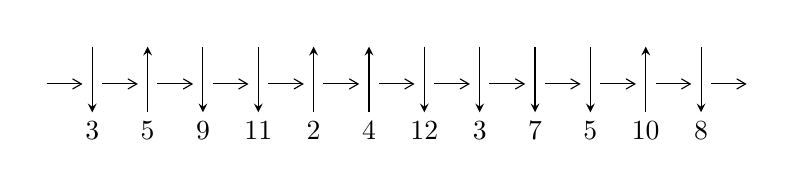
\begin{tikzpicture}[x=20pt, y=17pt]
	% nodes
	\node (C0) at (0, 0) {};
	\node (C1) at (1, 0) {};
	\node (C1U) at (1, +1) {};
	\node (C1D) at (1, -1) {3};

	\node (C2) at (2, 0) {};
	\node (C2U) at (2, +1) {};
	\node (C2D) at (2, -1) {5};

	\node (C3) at (3, 0) {};
	\node (C3U) at (3, +1) {};
	\node (C3D) at (3, -1) {9};

	\node (C4) at (4, 0) {};
	\node (C4U) at (4, +1) {};
	\node (C4D) at (4, -1) {11};

	\node (C5) at (5, 0) {};
	\node (C5U) at (5, +1) {};
	\node (C5D) at (5, -1) {2};

	\node (C6) at (6, 0) {};
	\node (C6U) at (6, +1) {};
	\node (C6D) at (6, -1) {4};

	\node (C7) at (7, 0) {};
	\node (C7U) at (7, +1) {};
	\node (C7D) at (7, -1) {12};

	\node (C8) at (8, 0) {};
	\node (C8U) at (8, +1) {};
	\node (C8D) at (8, -1) {3};

	\node (C9) at (9, 0) {};
	\node (C9U) at (9, +1) {};
	\node (C9D) at (9, -1) {7};

	\node (C10) at (10, 0) {};
	\node (C10U) at (10, +1) {};
	\node (C10D) at (10, -1) {5};

	\node (C11) at (11, 0) {};
	\node (C11U) at (11, +1) {};
	\node (C11D) at (11, -1) {10};

	\node (C12) at (12, 0) {};
	\node (C12U) at (12, +1) {};
	\node (C12D) at (12, -1) {8};
	\node (C13) at (13, 0) {};

	% arrows
	\draw[->,>={angle 60}]
	(C0) edge (C1) (C1) edge (C2) (C2) edge (C3) (C3) edge (C4) (C4) edge (C5) (C5) edge (C6) (C6) edge (C7) (C7) edge (C8) (C8) edge (C9) (C9) edge (C10) (C10) edge (C11) (C11) edge (C12) (C12) edge (C13) ;	\draw[->,>=stealth]
	(C1U) edge (C1D) (C2D) edge (C2U) (C3U) edge (C3D) (C4U) edge (C4D) (C5D) edge (C5U) (C6D) edge (C6U) (C7U) edge (C7D) (C8U) edge (C8D) (C9U) edge (C9D) (C10U) edge (C10D) (C11D) edge (C11U) (C12U) edge (C12D) ;
	\end{tikzpicture} \\
\hhline{~~} \\& 
\textbf{Solving Sequence} \\ \cline{2-2} 
 &
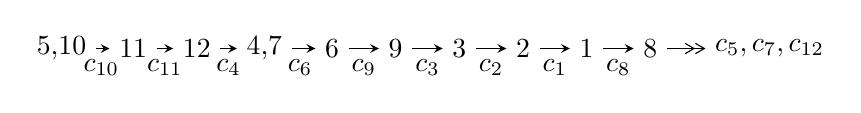
\begin{tikzpicture}[x=23pt, y=7pt]
	% node
	\node (A0) at (-1/8, 0) {5,10};
	\node (A1) at (1, 0) {11};
	\node (A2) at (2, 0) {12};
	\node (A3) at (49/16, 0) {4,7};
	\node (A4) at (33/8, 0) {6};
	\node (A5) at (41/8, 0) {9};
	\node (A6) at (49/8, 0) {3};
	\node (A7) at (57/8, 0) {2};
	\node (A8) at (65/8, 0) {1};
	\node (A9) at (73/8, 0) {8};
	\node (C1) at (1/2, -1) {$c_{10}$};
	\node (C2) at (3/2, -1) {$c_{11}$};
	\node (C3) at (5/2, -1) {$c_{4}$};
	\node (C4) at (29/8, -1) {$c_{6}$};
	\node (C5) at (37/8, -1) {$c_{9}$};
	\node (C6) at (45/8, -1) {$c_{3}$};
	\node (C7) at (53/8, -1) {$c_{2}$};
	\node (C8) at (61/8, -1) {$c_{1}$};
	\node (C9) at (69/8, -1) {$c_{8}$};
	\node (A10) at (11, 0) {$c_{5},c_{7},c_{12}$};

	% edge
	\draw[->,>=stealth]	
	(A0) edge (A1) (A1) edge (A2) (A2) edge (A3) (A3) edge (A4) (A4) edge (A5) (A5) edge (A6) (A6) edge (A7) (A7) edge (A8) (A8) edge (A9) ;
	\draw[->>,>={angle 60}]	
	(A9) edge (A10);
\end{tikzpicture} \\ 

\end{tabular} \\

\footnotetext{
The image of knot diagram is generated by the software ``\textbf{Draw programme}" developed by Andrew Bartholomew(\url{http://www.layer8.co.uk/maths/draw/index.htm\#Running-draw}), where we modified some parts for our purpose(\url{https://github.com/CATsTAILs/LinksPainter}).
}\phantom \\ \newline 
\centering \textbf{Ideals for irreducible components\footnotemark of $X_{\text{par}}$} 
 
\begin{align*}
I^u_{1}&=\langle 
-9 u^{16}+75 u^{15}+\cdots+4 b+48,\;-8 u^{16}+61 u^{15}+\cdots+4 a+16,\;u^{17}-9 u^{16}+\cdots-16 u+8\rangle \\
I^u_{2}&=\langle 
u^{12}+u^{11}+3 u^{10}+2 u^9+7 u^8+4 u^7+9 u^6+3 u^5+9 u^4+2 u^3+5 u^2+b+u+2,\\
\phantom{I^u_{2}}&\phantom{= \langle  }-3 u^{13}-3 u^{12}-8 u^{11}-5 u^{10}-18 u^9-10 u^8-23 u^7-8 u^6-23 u^5-6 u^4-14 u^3-4 u^2+a-5 u+1,\\
\phantom{I^u_{2}}&\phantom{= \langle  }u^{14}+u^{13}+3 u^{12}+2 u^{11}+7 u^{10}+4 u^9+10 u^8+4 u^7+11 u^6+3 u^5+8 u^4+2 u^3+4 u^2+1\rangle \\
\\
\end{align*}
\raggedright * 2 irreducible components of $\dim_{\mathbb{C}}=0$, with total 31 representations.\\
\footnotetext{All coefficients of polynomials are rational numbers. But the coefficients are sometimes approximated in decimal forms when there is not enough margin.}
\newpage
\renewcommand{\arraystretch}{1}
\centering \section*{I. $I^u_{1}= \langle -9 u^{16}+75 u^{15}+\cdots+4 b+48,\;-8 u^{16}+61 u^{15}+\cdots+4 a+16,\;u^{17}-9 u^{16}+\cdots-16 u+8 \rangle$}
\flushleft \textbf{(i) Arc colorings}\\
\begin{tabular}{m{7pt} m{180pt} m{7pt} m{180pt} }
\flushright $a_{5}=$&$\begin{pmatrix}0\\u\end{pmatrix}$ \\
\flushright $a_{10}=$&$\begin{pmatrix}1\\0\end{pmatrix}$ \\
\flushright $a_{11}=$&$\begin{pmatrix}1\\u^2\end{pmatrix}$ \\
\flushright $a_{12}=$&$\begin{pmatrix}u^2+1\\u^2\end{pmatrix}$ \\
\flushright $a_{4}=$&$\begin{pmatrix}u\\u^3+u\end{pmatrix}$ \\
\flushright $a_{7}=$&$\begin{pmatrix}2 u^{16}-\frac{61}{4} u^{15}+\cdots+\frac{53}{4} u-4\\\frac{9}{4} u^{16}-\frac{75}{4} u^{15}+\cdots+23 u-12\end{pmatrix}$ \\
\flushright $a_{6}=$&$\begin{pmatrix}-\frac{3}{2} u^{16}+\frac{45}{4} u^{15}+\cdots-\frac{35}{4} u+2\\-\frac{17}{4} u^{16}+\frac{151}{4} u^{15}+\cdots-51 u+34\end{pmatrix}$ \\
\flushright $a_{9}=$&$\begin{pmatrix}\frac{15}{8} u^{16}-\frac{117}{8} u^{15}+\cdots+14 u-\frac{5}{2}\\\frac{9}{4} u^{16}-\frac{77}{4} u^{15}+\cdots+\frac{55}{2} u-15\end{pmatrix}$ \\
\flushright $a_{3}=$&$\begin{pmatrix}\frac{1}{4} u^{16}-\frac{9}{4} u^{15}+\cdots+\frac{7}{2} u-\frac{5}{2}\\-\frac{1}{2} u^{15}+\frac{7}{2} u^{14}+\cdots+\frac{5}{2} u-2\end{pmatrix}$ \\
\flushright $a_{2}=$&$\begin{pmatrix}\frac{1}{4} u^{16}-\frac{9}{4} u^{15}+\cdots+\frac{7}{2} u-\frac{5}{2}\\-\frac{1}{2} u^{16}+3 u^{15}+\cdots+\frac{1}{2} u-2\end{pmatrix}$ \\
\flushright $a_{1}=$&$\begin{pmatrix}-\frac{13}{8} u^{16}+\frac{119}{8} u^{15}+\cdots-22 u+\frac{31}{2}\\\frac{5}{4} u^{16}-\frac{29}{4} u^{15}+\cdots-\frac{3}{2} u+11\end{pmatrix}$ \\
\flushright $a_{8}=$&$\begin{pmatrix}\frac{9}{4} u^{16}-18 u^{15}+\cdots+\frac{73}{4} u-6\\\frac{9}{4} u^{16}-\frac{79}{4} u^{15}+\cdots+29 u-16\end{pmatrix}$\\&\end{tabular}
\flushleft \textbf{(ii) Obstruction class $= -1$}\\~\\
\flushleft \textbf{(iii) Cusp Shapes $= -6 u^{16}+48 u^{15}-204 u^{14}+579 u^{13}-1201 u^{12}+1920 u^{11}-2456 u^{10}+2621 u^9-2430 u^8+2003 u^7-1452 u^6+891 u^5-445 u^4+148 u^3+6 u^2-44 u+10$}\\~\\
\newpage\renewcommand{\arraystretch}{1}
\flushleft \textbf{(iv) u-Polynomials at the component}\newline \\
\begin{tabular}{m{50pt}|m{274pt}}
Crossings & \hspace{64pt}u-Polynomials at each crossing \\
\hline $$\begin{aligned}c_{1}\end{aligned}$$&$\begin{aligned}
&u^{17}-22 u^{16}+\cdots+54 u-1
\end{aligned}$\\
\hline $$\begin{aligned}c_{2},c_{5}\end{aligned}$$&$\begin{aligned}
&u^{17}+2 u^{16}+\cdots-2 u+1
\end{aligned}$\\
\hline $$\begin{aligned}c_{3},c_{8}\end{aligned}$$&$\begin{aligned}
&u^{17}- u^{16}+\cdots- u+1
\end{aligned}$\\
\hline $$\begin{aligned}c_{4},c_{10}\end{aligned}$$&$\begin{aligned}
&u^{17}-9 u^{16}+\cdots-16 u+8
\end{aligned}$\\
\hline $$\begin{aligned}c_{6}\end{aligned}$$&$\begin{aligned}
&u^{17}+4 u^{16}+\cdots+24694 u+2511
\end{aligned}$\\
\hline $$\begin{aligned}c_{7},c_{12}\end{aligned}$$&$\begin{aligned}
&u^{17}+7 u^{15}+\cdots-226 u+111
\end{aligned}$\\
\hline $$\begin{aligned}c_{9}\end{aligned}$$&$\begin{aligned}
&u^{17}-3 u^{16}+\cdots-4 u+1
\end{aligned}$\\
\hline $$\begin{aligned}c_{11}\end{aligned}$$&$\begin{aligned}
&u^{17}-5 u^{16}+\cdots+160 u+64
\end{aligned}$\\
\hline
\end{tabular}\\~\\
\newpage\renewcommand{\arraystretch}{1}
\flushleft \textbf{(v) Riley Polynomials at the component}\newline \\
\begin{tabular}{m{50pt}|m{274pt}}
Crossings & \hspace{64pt}Riley Polynomials at each crossing \\
\hline $$\begin{aligned}c_{1}\end{aligned}$$&$\begin{aligned}
&y^{17}+62 y^{16}+\cdots+426 y-1
\end{aligned}$\\
\hline $$\begin{aligned}c_{2},c_{5}\end{aligned}$$&$\begin{aligned}
&y^{17}-22 y^{16}+\cdots+54 y-1
\end{aligned}$\\
\hline $$\begin{aligned}c_{3},c_{8}\end{aligned}$$&$\begin{aligned}
&y^{17}+21 y^{16}+\cdots-7 y-1
\end{aligned}$\\
\hline $$\begin{aligned}c_{4},c_{10}\end{aligned}$$&$\begin{aligned}
&y^{17}+5 y^{16}+\cdots+160 y-64
\end{aligned}$\\
\hline $$\begin{aligned}c_{6}\end{aligned}$$&$\begin{aligned}
&y^{17}-22 y^{16}+\cdots+769543456 y-6305121
\end{aligned}$\\
\hline $$\begin{aligned}c_{7},c_{12}\end{aligned}$$&$\begin{aligned}
&y^{17}+14 y^{16}+\cdots-22850 y-12321
\end{aligned}$\\
\hline $$\begin{aligned}c_{9}\end{aligned}$$&$\begin{aligned}
&y^{17}-3 y^{16}+\cdots+10 y-1
\end{aligned}$\\
\hline $$\begin{aligned}c_{11}\end{aligned}$$&$\begin{aligned}
&y^{17}+13 y^{16}+\cdots+156160 y-4096
\end{aligned}$\\
\hline
\end{tabular}\\~\\
\newpage\flushleft \textbf{(vi) Complex Volumes and Cusp Shapes}
$$\begin{array}{c|c|c}  
\text{Solutions to }I^u_{1}& \I (\text{vol} + \sqrt{-1}CS) & \text{Cusp shape}\\
 \hline 
\begin{aligned}
u &= \phantom{-}0.743107 + 0.737300 I \\
a &= -0.957729 + 0.743386 I \\
b &= -1.065040 + 0.659072 I\end{aligned}
 & -3.59959 + 0.58481 I & -8.87613 + 1.72757 I \\ \hline\begin{aligned}
u &= \phantom{-}0.743107 - 0.737300 I \\
a &= -0.957729 - 0.743386 I \\
b &= -1.065040 - 0.659072 I\end{aligned}
 & -3.59959 - 0.58481 I & -8.87613 - 1.72757 I \\ \hline\begin{aligned}
u &= -0.072889 + 0.887618 I \\
a &= \phantom{-}0.312452 - 0.912707 I \\
b &= -0.304982 + 0.710279 I\end{aligned}
 & \phantom{-}1.67215 + 1.49188 I & \phantom{-}1.61333 - 4.98502 I \\ \hline\begin{aligned}
u &= -0.072889 - 0.887618 I \\
a &= \phantom{-}0.312452 + 0.912707 I \\
b &= -0.304982 - 0.710279 I\end{aligned}
 & \phantom{-}1.67215 - 1.49188 I & \phantom{-}1.61333 + 4.98502 I \\ \hline\begin{aligned}
u &= -0.474839 + 0.714353 I \\
a &= \phantom{-}1.293010 + 0.446550 I \\
b &= \phantom{-}0.470362 - 0.202610 I\end{aligned}
 & -0.29498 + 1.80975 I & -2.70110 - 3.65617 I \\ \hline\begin{aligned}
u &= -0.474839 - 0.714353 I \\
a &= \phantom{-}1.293010 - 0.446550 I \\
b &= \phantom{-}0.470362 + 0.202610 I\end{aligned}
 & -0.29498 - 1.80975 I & -2.70110 + 3.65617 I \\ \hline\begin{aligned}
u &= \phantom{-}0.699430 + 0.964772 I \\
a &= -1.65451 + 0.74282 I \\
b &= -1.001640 - 0.878315 I\end{aligned}
 & -2.90799 - 6.08549 I & -5.32420 + 3.68722 I \\ \hline\begin{aligned}
u &= \phantom{-}0.699430 - 0.964772 I \\
a &= -1.65451 - 0.74282 I \\
b &= -1.001640 + 0.878315 I\end{aligned}
 & -2.90799 + 6.08549 I & -5.32420 - 3.68722 I \\ \hline\begin{aligned}
u &= \phantom{-}0.864249 + 0.915420 I \\
a &= \phantom{-}1.71758 - 0.46850 I \\
b &= \phantom{-}0.779025 + 0.016840 I\end{aligned}
 & -7.95991 - 3.20234 I & -15.1724 + 0.4148 I \\ \hline\begin{aligned}
u &= \phantom{-}0.864249 - 0.915420 I \\
a &= \phantom{-}1.71758 + 0.46850 I \\
b &= \phantom{-}0.779025 - 0.016840 I\end{aligned}
 & -7.95991 + 3.20234 I & -15.1724 - 0.4148 I\\
 \hline 
 \end{array}$$\newpage$$\begin{array}{c|c|c}  
\text{Solutions to }I^u_{1}& \I (\text{vol} + \sqrt{-1}CS) & \text{Cusp shape}\\
 \hline 
\begin{aligned}
u &= \phantom{-}1.408880 + 0.063065 I \\
a &= \phantom{-}1.183850 - 0.166931 I \\
b &= \phantom{-}0.955388 - 0.931462 I\end{aligned}
 & \phantom{-}6.30330 + 3.42896 I & -6.06062 - 2.16109 I \\ \hline\begin{aligned}
u &= \phantom{-}1.408880 - 0.063065 I \\
a &= \phantom{-}1.183850 + 0.166931 I \\
b &= \phantom{-}0.955388 + 0.931462 I\end{aligned}
 & \phantom{-}6.30330 - 3.42896 I & -6.06062 + 2.16109 I \\ \hline\begin{aligned}
u &= -0.395985\phantom{ +0.000000I} \\
a &= -0.300112\phantom{ +0.000000I} \\
b &= -0.572653\phantom{ +0.000000I}\end{aligned}
 & -0.874933\phantom{ +0.000000I} & -11.5210\phantom{ +0.000000I} \\ \hline\begin{aligned}
u &= \phantom{-}0.72984 + 1.44188 I \\
a &= \phantom{-}0.168023 - 0.244503 I \\
b &= \phantom{-}0.909775 - 1.029340 I\end{aligned}
 & \phantom{-}10.83540 - 3.92897 I & -4.57004 + 0.99423 I \\ \hline\begin{aligned}
u &= \phantom{-}0.72984 - 1.44188 I \\
a &= \phantom{-}0.168023 + 0.244503 I \\
b &= \phantom{-}0.909775 + 1.029340 I\end{aligned}
 & \phantom{-}10.83540 + 3.92897 I & -4.57004 - 0.99423 I \\ \hline\begin{aligned}
u &= \phantom{-}0.80021 + 1.43594 I \\
a &= \phantom{-}1.33738 - 0.75405 I \\
b &= \phantom{-}1.043440 + 0.934400 I\end{aligned}
 & \phantom{-}10.3710 - 11.0996 I & -5.14830 + 4.90846 I \\ \hline\begin{aligned}
u &= \phantom{-}0.80021 - 1.43594 I \\
a &= \phantom{-}1.33738 + 0.75405 I \\
b &= \phantom{-}1.043440 - 0.934400 I\end{aligned}
 & \phantom{-}10.3710 + 11.0996 I & -5.14830 - 4.90846 I\\
 \hline 
 \end{array}$$\newpage\newpage\renewcommand{\arraystretch}{1}
\centering \section*{II. $I^u_{2}= \langle u^{12}+u^{11}+\cdots+b+2,\;-3 u^{13}-3 u^{12}+\cdots+a+1,\;u^{14}+u^{13}+\cdots+4 u^2+1 \rangle$}
\flushleft \textbf{(i) Arc colorings}\\
\begin{tabular}{m{7pt} m{180pt} m{7pt} m{180pt} }
\flushright $a_{5}=$&$\begin{pmatrix}0\\u\end{pmatrix}$ \\
\flushright $a_{10}=$&$\begin{pmatrix}1\\0\end{pmatrix}$ \\
\flushright $a_{11}=$&$\begin{pmatrix}1\\u^2\end{pmatrix}$ \\
\flushright $a_{12}=$&$\begin{pmatrix}u^2+1\\u^2\end{pmatrix}$ \\
\flushright $a_{4}=$&$\begin{pmatrix}u\\u^3+u\end{pmatrix}$ \\
\flushright $a_{7}=$&$\begin{pmatrix}3 u^{13}+3 u^{12}+\cdots+5 u-1\\- u^{12}- u^{11}+\cdots- u-2\end{pmatrix}$ \\
\flushright $a_{6}=$&$\begin{pmatrix}2 u^{13}+2 u^{12}+\cdots+3 u-2\\- u^{13}-2 u^{12}+\cdots-2 u-3\end{pmatrix}$ \\
\flushright $a_{9}=$&$\begin{pmatrix}2 u^{13}+2 u^{12}+\cdots+2 u-3\\- u^{12}-2 u^{11}+\cdots-3 u-2\end{pmatrix}$ \\
\flushright $a_{3}=$&$\begin{pmatrix}u^{12}+u^{11}+\cdots+2 u+3\\u^{13}+u^{12}+\cdots+u^2+4 u\end{pmatrix}$ \\
\flushright $a_{2}=$&$\begin{pmatrix}u^{12}+u^{11}+\cdots+2 u+3\\u^{13}+u^{12}+\cdots+4 u-1\end{pmatrix}$ \\
\flushright $a_{1}=$&$\begin{pmatrix}-2 u^{13}-2 u^{12}+\cdots-5 u+1\\- u^{13}- u^{12}+\cdots-3 u^2+u\end{pmatrix}$ \\
\flushright $a_{8}=$&$\begin{pmatrix}2 u^{13}+3 u^{12}+\cdots+4 u-1\\- u^{12}- u^{11}+\cdots-8 u^2-3\end{pmatrix}$\\&\end{tabular}
\flushleft \textbf{(ii) Obstruction class $= 1$}\\~\\
\flushleft \textbf{(iii) Cusp Shapes $= - u^{13}+3 u^{12}+2 u^{11}+12 u^{10}+9 u^9+32 u^8+21 u^7+42 u^6+25 u^5+45 u^4+22 u^3+24 u^2+10 u$}\\~\\
\newpage\renewcommand{\arraystretch}{1}
\flushleft \textbf{(iv) u-Polynomials at the component}\newline \\
\begin{tabular}{m{50pt}|m{274pt}}
Crossings & \hspace{64pt}u-Polynomials at each crossing \\
\hline $$\begin{aligned}c_{1}\end{aligned}$$&$\begin{aligned}
&u^{14}-11 u^{13}+\cdots-4 u+1
\end{aligned}$\\
\hline $$\begin{aligned}c_{2}\end{aligned}$$&$\begin{aligned}
&u^{14}+u^{13}+6 u^{12}+4 u^{11}+9 u^{10}+3 u^8-5 u^7-4 u^5+2 u^4- u^3+2 u^2+1
\end{aligned}$\\
\hline $$\begin{aligned}c_{3}\end{aligned}$$&$\begin{aligned}
&u^{14}-5 u^{12}+9 u^{10}-2 u^9-6 u^8+6 u^7-7 u^5+4 u^4+4 u^3-3 u^2- u+1
\end{aligned}$\\
\hline $$\begin{aligned}c_{4}\end{aligned}$$&$\begin{aligned}
&u^{14}- u^{13}+\cdots+4 u^2+1
\end{aligned}$\\
\hline $$\begin{aligned}c_{5}\end{aligned}$$&$\begin{aligned}
&u^{14}- u^{13}+6 u^{12}-4 u^{11}+9 u^{10}+3 u^8+5 u^7+4 u^5+2 u^4+u^3+2 u^2+1
\end{aligned}$\\
\hline $$\begin{aligned}c_{6}\end{aligned}$$&$\begin{aligned}
&u^{14}- u^{13}+\cdots+8 u+67
\end{aligned}$\\
\hline $$\begin{aligned}c_{7}\end{aligned}$$&$\begin{aligned}
&u^{14}- u^{13}+\cdots+4 u+1
\end{aligned}$\\
\hline $$\begin{aligned}c_{8}\end{aligned}$$&$\begin{aligned}
&u^{14}-5 u^{12}+9 u^{10}+2 u^9-6 u^8-6 u^7+7 u^5+4 u^4-4 u^3-3 u^2+u+1
\end{aligned}$\\
\hline $$\begin{aligned}c_{9}\end{aligned}$$&$\begin{aligned}
&u^{14}+6 u^{13}+\cdots+4 u+1
\end{aligned}$\\
\hline $$\begin{aligned}c_{10}\end{aligned}$$&$\begin{aligned}
&u^{14}+u^{13}+\cdots+4 u^2+1
\end{aligned}$\\
\hline $$\begin{aligned}c_{11}\end{aligned}$$&$\begin{aligned}
&u^{14}-5 u^{13}+\cdots-8 u+1
\end{aligned}$\\
\hline $$\begin{aligned}c_{12}\end{aligned}$$&$\begin{aligned}
&u^{14}+u^{13}+\cdots-4 u+1
\end{aligned}$\\
\hline
\end{tabular}\\~\\
\newpage\renewcommand{\arraystretch}{1}
\flushleft \textbf{(v) Riley Polynomials at the component}\newline \\
\begin{tabular}{m{50pt}|m{274pt}}
Crossings & \hspace{64pt}Riley Polynomials at each crossing \\
\hline $$\begin{aligned}c_{1}\end{aligned}$$&$\begin{aligned}
&y^{14}-29 y^{13}+\cdots+12 y^2+1
\end{aligned}$\\
\hline $$\begin{aligned}c_{2},c_{5}\end{aligned}$$&$\begin{aligned}
&y^{14}+11 y^{13}+\cdots+4 y+1
\end{aligned}$\\
\hline $$\begin{aligned}c_{3},c_{8}\end{aligned}$$&$\begin{aligned}
&y^{14}-10 y^{13}+\cdots-7 y+1
\end{aligned}$\\
\hline $$\begin{aligned}c_{4},c_{10}\end{aligned}$$&$\begin{aligned}
&y^{14}+5 y^{13}+\cdots+8 y+1
\end{aligned}$\\
\hline $$\begin{aligned}c_{6}\end{aligned}$$&$\begin{aligned}
&y^{14}+11 y^{13}+\cdots-466 y+4489
\end{aligned}$\\
\hline $$\begin{aligned}c_{7},c_{12}\end{aligned}$$&$\begin{aligned}
&y^{14}-13 y^{13}+\cdots-4 y+1
\end{aligned}$\\
\hline $$\begin{aligned}c_{9}\end{aligned}$$&$\begin{aligned}
&y^{14}-2 y^{13}+\cdots-8 y+1
\end{aligned}$\\
\hline $$\begin{aligned}c_{11}\end{aligned}$$&$\begin{aligned}
&y^{14}+13 y^{13}+\cdots+32 y^2+1
\end{aligned}$\\
\hline
\end{tabular}\\~\\
\newpage\flushleft \textbf{(vi) Complex Volumes and Cusp Shapes}
$$\begin{array}{c|c|c}  
\text{Solutions to }I^u_{2}& \I (\text{vol} + \sqrt{-1}CS) & \text{Cusp shape}\\
 \hline 
\begin{aligned}
u &= \phantom{-}0.105110 + 0.959669 I \\
a &= \phantom{-}0.448698 - 0.035015 I \\
b &= -0.594085 + 0.956154 I\end{aligned}
 & \phantom{-}0.09953 + 1.96463 I & -3.48083 - 3.91633 I \\ \hline\begin{aligned}
u &= \phantom{-}0.105110 - 0.959669 I \\
a &= \phantom{-}0.448698 + 0.035015 I \\
b &= -0.594085 - 0.956154 I\end{aligned}
 & \phantom{-}0.09953 - 1.96463 I & -3.48083 + 3.91633 I \\ \hline\begin{aligned}
u &= \phantom{-}0.694518 + 0.776039 I \\
a &= -0.573318 + 1.021770 I \\
b &= -1.16230 + 0.95610 I\end{aligned}
 & -3.84339 + 1.43715 I & -12.12204 - 5.82210 I \\ \hline\begin{aligned}
u &= \phantom{-}0.694518 - 0.776039 I \\
a &= -0.573318 - 1.021770 I \\
b &= -1.16230 - 0.95610 I\end{aligned}
 & -3.84339 - 1.43715 I & -12.12204 + 5.82210 I \\ \hline\begin{aligned}
u &= -0.584040 + 0.656749 I \\
a &= \phantom{-}0.75333 - 1.27705 I \\
b &= \phantom{-}0.796480 + 0.277469 I\end{aligned}
 & -6.62904 + 0.87099 I & -9.32156 + 1.93932 I \\ \hline\begin{aligned}
u &= -0.584040 - 0.656749 I \\
a &= \phantom{-}0.75333 + 1.27705 I \\
b &= \phantom{-}0.796480 - 0.277469 I\end{aligned}
 & -6.62904 - 0.87099 I & -9.32156 - 1.93932 I \\ \hline\begin{aligned}
u &= \phantom{-}0.672935 + 0.942423 I \\
a &= -1.78530 + 0.66319 I \\
b &= -1.09781 - 1.12323 I\end{aligned}
 & -3.32221 - 6.71387 I & -11.7069 + 12.3294 I \\ \hline\begin{aligned}
u &= \phantom{-}0.672935 - 0.942423 I \\
a &= -1.78530 - 0.66319 I \\
b &= -1.09781 + 1.12323 I\end{aligned}
 & -3.32221 + 6.71387 I & -11.7069 - 12.3294 I \\ \hline\begin{aligned}
u &= -0.645970 + 1.039580 I \\
a &= \phantom{-}0.263318 + 0.909593 I \\
b &= \phantom{-}0.491954 - 0.568665 I\end{aligned}
 & -5.34937 + 4.06327 I & -5.63140 - 4.63388 I \\ \hline\begin{aligned}
u &= -0.645970 - 1.039580 I \\
a &= \phantom{-}0.263318 - 0.909593 I \\
b &= \phantom{-}0.491954 + 0.568665 I\end{aligned}
 & -5.34937 - 4.06327 I & -5.63140 + 4.63388 I\\
 \hline 
 \end{array}$$\newpage$$\begin{array}{c|c|c}  
\text{Solutions to }I^u_{2}& \I (\text{vol} + \sqrt{-1}CS) & \text{Cusp shape}\\
 \hline 
\begin{aligned}
u &= -0.925465 + 0.908624 I \\
a &= -1.45765 - 0.16567 I \\
b &= -0.528256 + 0.113442 I\end{aligned}
 & -7.43274 + 3.38328 I & -1.12875 - 4.65800 I \\ \hline\begin{aligned}
u &= -0.925465 - 0.908624 I \\
a &= -1.45765 + 0.16567 I \\
b &= -0.528256 - 0.113442 I\end{aligned}
 & -7.43274 - 3.38328 I & -1.12875 + 4.65800 I \\ \hline\begin{aligned}
u &= \phantom{-}0.182913 + 0.587851 I \\
a &= -2.14907 + 1.62071 I \\
b &= -0.905989 - 0.618123 I\end{aligned}
 & -1.48665 - 3.24685 I & -5.60851 + 4.03314 I \\ \hline\begin{aligned}
u &= \phantom{-}0.182913 - 0.587851 I \\
a &= -2.14907 - 1.62071 I \\
b &= -0.905989 + 0.618123 I\end{aligned}
 & -1.48665 + 3.24685 I & -5.60851 - 4.03314 I\\
 \hline 
 \end{array}$$\newpage
\newpage\renewcommand{\arraystretch}{1}
\centering \section*{ III. u-Polynomials}
\begin{tabular}{m{50pt}|m{274pt}}
Crossings & \hspace{64pt}u-Polynomials at each crossing \\
\hline $$\begin{aligned}c_{1}\end{aligned}$$&$\begin{aligned}
&(u^{14}-11 u^{13}+\cdots-4 u+1)(u^{17}-22 u^{16}+\cdots+54 u-1)
\end{aligned}$\\
\hline $$\begin{aligned}c_{2}\end{aligned}$$&$\begin{aligned}
&(u^{14}+u^{13}+6 u^{12}+4 u^{11}+9 u^{10}+3 u^8-5 u^7-4 u^5+2 u^4- u^3+2 u^2+1)\\
&\cdot(u^{17}+2 u^{16}+\cdots-2 u+1)
\end{aligned}$\\
\hline $$\begin{aligned}c_{3}\end{aligned}$$&$\begin{aligned}
&(u^{14}-5 u^{12}+9 u^{10}-2 u^9-6 u^8+6 u^7-7 u^5+4 u^4+4 u^3-3 u^2- u+1)\\
&\cdot(u^{17}- u^{16}+\cdots- u+1)
\end{aligned}$\\
\hline $$\begin{aligned}c_{4}\end{aligned}$$&$\begin{aligned}
&(u^{14}- u^{13}+\cdots+4 u^2+1)(u^{17}-9 u^{16}+\cdots-16 u+8)
\end{aligned}$\\
\hline $$\begin{aligned}c_{5}\end{aligned}$$&$\begin{aligned}
&(u^{14}- u^{13}+6 u^{12}-4 u^{11}+9 u^{10}+3 u^8+5 u^7+4 u^5+2 u^4+u^3+2 u^2+1)\\
&\cdot(u^{17}+2 u^{16}+\cdots-2 u+1)
\end{aligned}$\\
\hline $$\begin{aligned}c_{6}\end{aligned}$$&$\begin{aligned}
&(u^{14}- u^{13}+\cdots+8 u+67)(u^{17}+4 u^{16}+\cdots+24694 u+2511)
\end{aligned}$\\
\hline $$\begin{aligned}c_{7}\end{aligned}$$&$\begin{aligned}
&(u^{14}- u^{13}+\cdots+4 u+1)(u^{17}+7 u^{15}+\cdots-226 u+111)
\end{aligned}$\\
\hline $$\begin{aligned}c_{8}\end{aligned}$$&$\begin{aligned}
&(u^{14}-5 u^{12}+9 u^{10}+2 u^9-6 u^8-6 u^7+7 u^5+4 u^4-4 u^3-3 u^2+u+1)\\
&\cdot(u^{17}- u^{16}+\cdots- u+1)
\end{aligned}$\\
\hline $$\begin{aligned}c_{9}\end{aligned}$$&$\begin{aligned}
&(u^{14}+6 u^{13}+\cdots+4 u+1)(u^{17}-3 u^{16}+\cdots-4 u+1)
\end{aligned}$\\
\hline $$\begin{aligned}c_{10}\end{aligned}$$&$\begin{aligned}
&(u^{14}+u^{13}+\cdots+4 u^2+1)(u^{17}-9 u^{16}+\cdots-16 u+8)
\end{aligned}$\\
\hline $$\begin{aligned}c_{11}\end{aligned}$$&$\begin{aligned}
&(u^{14}-5 u^{13}+\cdots-8 u+1)(u^{17}-5 u^{16}+\cdots+160 u+64)
\end{aligned}$\\
\hline $$\begin{aligned}c_{12}\end{aligned}$$&$\begin{aligned}
&(u^{14}+u^{13}+\cdots-4 u+1)(u^{17}+7 u^{15}+\cdots-226 u+111)
\end{aligned}$\\
\hline
\end{tabular}\newpage\renewcommand{\arraystretch}{1}
\centering \section*{ IV. Riley Polynomials}
\begin{tabular}{m{50pt}|m{274pt}}
Crossings & \hspace{64pt}Riley Polynomials at each crossing \\
\hline $$\begin{aligned}c_{1}\end{aligned}$$&$\begin{aligned}
&(y^{14}-29 y^{13}+\cdots+12 y^2+1)(y^{17}+62 y^{16}+\cdots+426 y-1)
\end{aligned}$\\
\hline $$\begin{aligned}c_{2},c_{5}\end{aligned}$$&$\begin{aligned}
&(y^{14}+11 y^{13}+\cdots+4 y+1)(y^{17}-22 y^{16}+\cdots+54 y-1)
\end{aligned}$\\
\hline $$\begin{aligned}c_{3},c_{8}\end{aligned}$$&$\begin{aligned}
&(y^{14}-10 y^{13}+\cdots-7 y+1)(y^{17}+21 y^{16}+\cdots-7 y-1)
\end{aligned}$\\
\hline $$\begin{aligned}c_{4},c_{10}\end{aligned}$$&$\begin{aligned}
&(y^{14}+5 y^{13}+\cdots+8 y+1)(y^{17}+5 y^{16}+\cdots+160 y-64)
\end{aligned}$\\
\hline $$\begin{aligned}c_{6}\end{aligned}$$&$\begin{aligned}
&(y^{14}+11 y^{13}+\cdots-466 y+4489)\\
&\cdot(y^{17}-22 y^{16}+\cdots+769543456 y-6305121)
\end{aligned}$\\
\hline $$\begin{aligned}c_{7},c_{12}\end{aligned}$$&$\begin{aligned}
&(y^{14}-13 y^{13}+\cdots-4 y+1)(y^{17}+14 y^{16}+\cdots-22850 y-12321)
\end{aligned}$\\
\hline $$\begin{aligned}c_{9}\end{aligned}$$&$\begin{aligned}
&(y^{14}-2 y^{13}+\cdots-8 y+1)(y^{17}-3 y^{16}+\cdots+10 y-1)
\end{aligned}$\\
\hline $$\begin{aligned}c_{11}\end{aligned}$$&$\begin{aligned}
&(y^{14}+13 y^{13}+\cdots+32 y^2+1)(y^{17}+13 y^{16}+\cdots+156160 y-4096)
\end{aligned}$\\
\hline
\end{tabular}
\vskip 2pc
\end{document}